\documentclass [a4paper,final,conference,10pt]{IDAACS}
\usepackage[utf8]{inputenc}
\usepackage[english]{babel}
\usepackage{amsmath}
\usepackage{graphicx}
\usepackage{multirow}
\usepackage{cite}
\usepackage{pgfplots}
\usepackage{pgfplotstable}
%\title{Effective Parallelization of Mixed-Critical Software to Distributed Heterogeneous Mutlicoresystems}
%\subtitle{
%	Approaching Challenges of Automotive Constrains: Partial Realtime, Safety, Affinity and Connectivity}
%Bare-Metal and OS-based 
%\title{Constrained Parallelization of Mixed-Critical Applications to Distributed Heterogeneous Hardware}
\title{Constrained Mixed-Critical Parallelization for Distributed Heterogeneous Systems}
\author{
	No authors given for review
%\IEEEauthorblockN{Robert Höttger, Mustafa Özcelikörs, Philipp Heisig, Lukas Krawczyk, Carsten Wolff, Burkhard Igel}
%						Third Author's Name\IEEEauthorrefmark{2}}
%\IEEEauthorblockA{IDiAL Institute - Dortmund University of Applied Sciences and Arts, \\\{robert.hoettger, mustafa.ozcelikors, lukas.krawczyk,  philipp.heisig, carsten.wolff, igel\}@fh-dortmund.de \\ www.idial.institute 
%						\IEEEauthorrefmark{2}Affiliation, Postal address, e-mail, Web address (URL)\\
%						\IEEEauthorrefmark{3}Affiliation, Postal address, e-mail, Web address (URL)\\
%	}
}
\begin{document}
\maketitle

\let\thefootnote\relax\footnotetext{As part of the AMALTHEA4public project, this work has been funded by the German Federal Ministry of Education and Research - BMBF, under funding no. $01|S14029K$}

\begin{abstract}
%TODO focus on responsiveness or automatic constrained parallelization 
Distributing software effectively to multi core, many core, and distributed systems has been studied for decades but still advances successively driven by domain specific constraints. 
Programming vehicle ECUs is one of the most constrained domains that %just
recently approached the need for concurrency due to advanced driver assistant systems or autonomous driving approaches. 

In this paper, software distribution challenges for such systems are discussed and solutions are presented upon instruction precise modeling, affinity constrained distribution, and reducing task response times achieved by advanced software parallelization. 
%The solutions are compared with OS-based and sequential implementations while considering fixed priorities for %sequential, OS based, and APP4MC scheduling.
%two platform's default scheduling algorithms as well as various constraints.
%round-robin and CFS scheduling and 
%The latter case has been described and published already but 
Therefore, existing partitioning and mapping algorithms are advanced to consider affinity constraints, software component tags and communication costs.
%related mapping described in this paper.
Our experiments along a remote controlled model car show that using our new advanced results instead of sequential implementations or software distributions provided by the operating system
%-based software distributions 
on a distributed heterogeneous system %outperforms available approaches 
significantly improves its responsiveness in order to potentially reduce energy consumption and replaces error prone manual constraint considerations for mixed-critical applications.  
%TODO percent
\end{abstract}

\begin{IEEEkeywords}
Constrained parallelization, heterogeneous systems, distributed systems, multicore, parallel embedded systems
\end{IEEEkeywords}

\section{Introduction}
Developing software for the automotive domain requires the consideration of many constraints originating from safety, security, timing, or similar requirements. In addition, established processes such as verification, validation, testing, simulation, and product line engineering as well as consulting various architectures, standards, models, and assessments regarding consistent, modular, and scalable software require dozens of tools. Corresponding tool efforts further lack in transparency and hence impede to comprehensively conceive applications. 

Recent approaches such as APP4MC\cite{app4mc}
%\footnote{\underline{A}pplication \underline{P}latform \underline{P}roject for Multi and Manycore, http://eclip.se/a7, access February 2017} 
address related challenges. APP4MC specifically provides a common adaptable platform based on AUTOSAR\cite{autosar} and includes a standardized data model. Any specific commercial or proprietary tooling can be integrated in order to address the seamless interaction between tools. This significantly eases development processes e.g. when concerning product line management, requirements engineering, traceability, testing or the verification of partitioning, mapping, and more. Consequently, we use the open source APP4MC environment and its parallelization features in this paper for the purpose of addressing both industrial and research related models. New results are not only evaluated in terms of model analysis but also validated among a specific use case described in Section \ref{sec:rccar}. 

The further remainder of this paper is structured as follows: Section \ref{sec:rccar} illustrates capabilities and properties of the A4MCAR demonstrator as well as its distributed architecture and concurrency capabilities. Afterwards, Section \ref{sec:app4mc} roughly describes the environment this contribution is based upon and its specifics among constraints and instructions. Subsequently, Section \ref{sec:eval} evaluates the results and benefits gained from adapting APP4MC parallelization features for automatic and constraint based software distributions of a mixed critical application, while Section \ref{sec:relatedWork} reviews related work.  %outlines the specific developments and solutions to precise modeling and software parallelization that is evaluated and compared to related approaches in section \ref{sec:eval}. 
Finally, Section \ref{sec:concl} concludes this paper's contributions and discusses benefits, disadvantages, possible extensions, and promising outlooks that potentially advance the current approach.

\section{A4MCAR}
\label{sec:rccar}
The A4MCAR primarily serves validating results received from the adapted software distribution results of APP4MC. It consists of 16 100MHz logical cores on a XMOS xCORE-200 eXplorerKIT (XS-1) device and
%2 instructions per cycle see (more details): https://www.xmos.com/download/private/xCORE-Architecture-Flyer%281.1%29.pdf
%2000MIPS 16 core: https://www.xmos.com/download/private/xCORE-200-XE-Product-Brief%281.2%29.pdf
%--> 125MIPS per logical core, --> 1,25 instructions per cycle?
%combined with 
four cores clocked at 1200MHz on a Raspberry Pi 3 (ARM Coretex-A53). With using APP4MC, we show that automatic software distributions provided by the operating system(s) do not always create the most efficient results.
The current Raspberry Pi distribution includes processes for the touchscreen, ethernet communication, core utilization reader, mjpg streamer, vnc application for remote server data exchange, apache2, OpenCV\cite{opencv} image processing, and additional cyclewasters. The latter processes perform matrix multiplications ans can be started on the RPI in order to push the core utilization to a maximum and consider high workload. The effective distribution by APP4MC is crucial to provide deadline violation free program execution. 
\begin{figure}[h!]
	\centering
	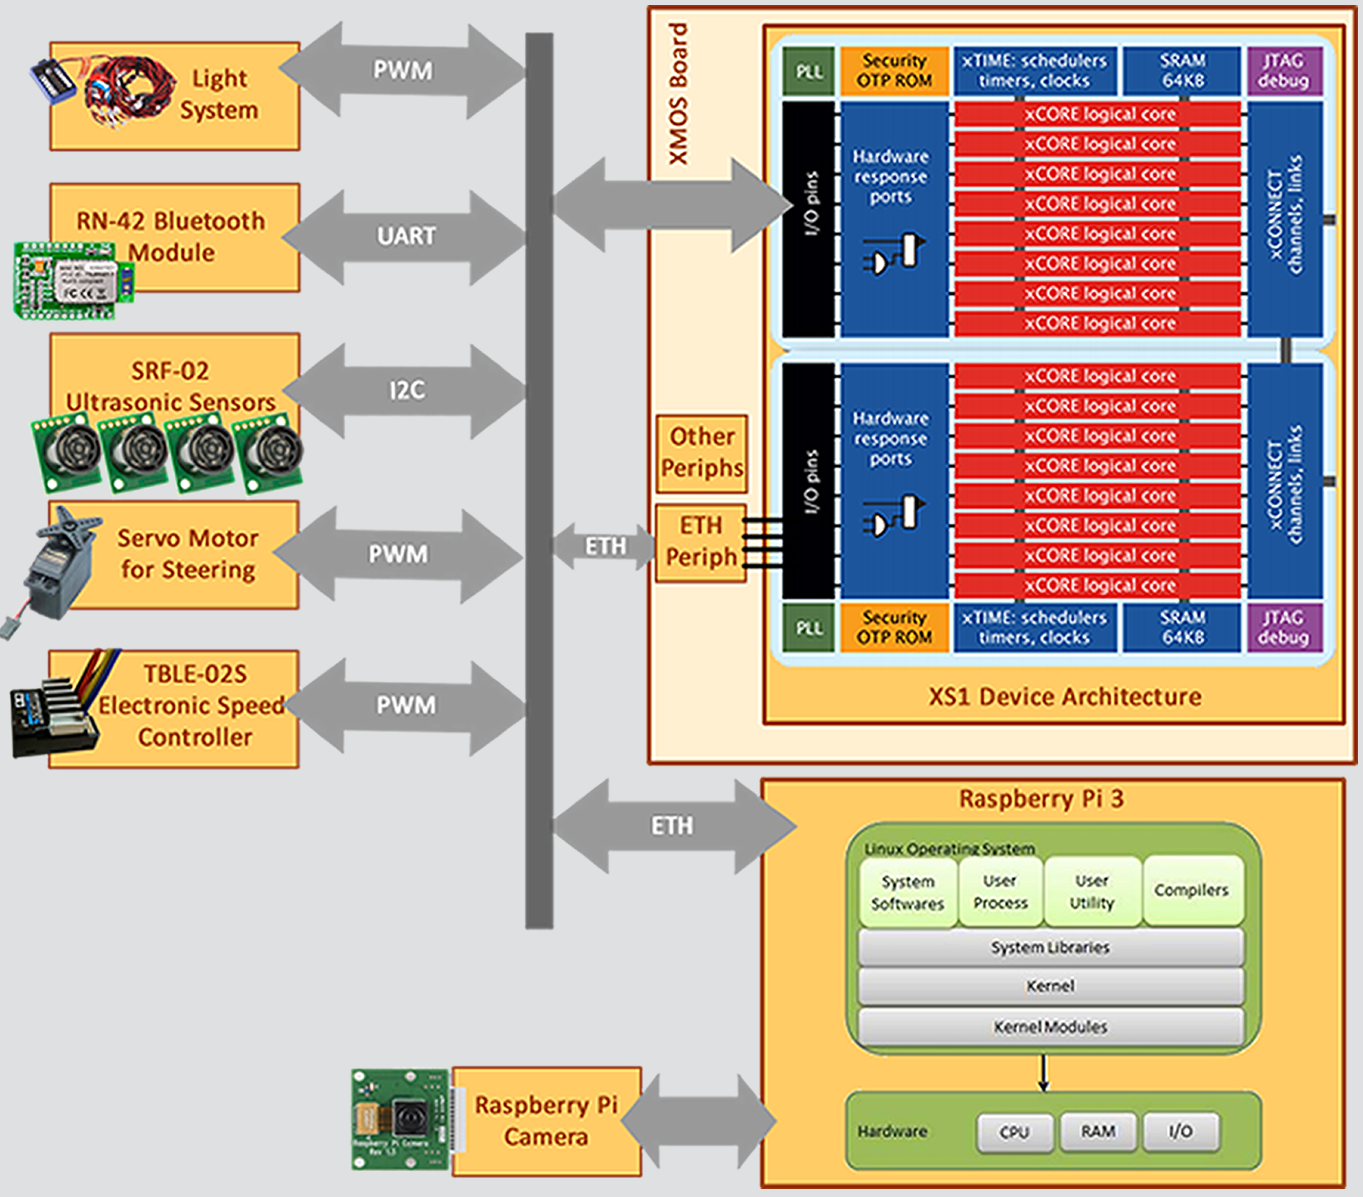
\includegraphics[scale=0.1]{images/hwarch.png}
	\caption{\label{fig:arch}A4MCAR architecture, interfaces, sensors, and actuators}
\end{figure}
The XMOS tasks focus on necessary real time implementations. Scheduling on the XMOS is non preemptive and allows a better determinism as well as easier \underline{W}orst \underline{C}ase \underline{E}xecution \underline{T}ime (WCET) reasoning due to less context switching and less scheduling jitter \cite{xmos}. However, since our number of tasks exceed the total number of available cores on the XMOS, we had to define high priority tasks, that run on dedicated cores, and low priority tasks that run concurrently with other low level tasks in cooperative multitask manner on common cores (via \textit{combinable} functions in XMOS terminology). The amount of high priority tasks thereby defines the number of cores available for the low priority tasks. 

Figure \ref{fig:arch} shows the basic A4MCAR architecture that uses different communication APIs such as Ethernet, I2C, or UART as well as various actuators and sensors to interact with its environment. Its current application is to approach autonomous driving scenarios.

\section{APP4MC}
\label{sec:app4mc}
%FOCUS Constraints
APP4MC is an open source project for developing multi and many core systems primarily for the automotive domain. Instead of describing its different purposes and features, this section focuses on the required steps to utilize APP4MC parallelization capabilities \cite{ICPDSSE}, i.e. partitioning and mapping. Those processes have been advanced in recent years to consider affinity, allocation, and safety constraints among others. 

Manual constraint considerations are usually error prone, time consuming, and rather complex and substantially affect responsiveness, i.e. timing effectiveness as well as logical correct software execution. Adapting partitioning and mapping towards those constraints has shown that such considerations and result validation, e.g. regarding deadlines, can be done automatically. Hence, constrained software developments of mixed-critical applications for distributed heterogeneous multi core systems are significantly eased.% and results improve the target's responsiveness when using APP4MC.

Dealing with safety constraints ensures that tasks with a specific \underline{A}utomotive \underline{S}afety \underline{I}ntegrity \underline{L}evel (ASIL) are allocated to processing units (cores) featuring the corresponding ASIL level. Allocation constraints are considered the same way, except that instead of ASIL levels properties such as \underline{F}loating \underline{P}oint \underline{U}nit (FPU) connectivity, cache memory size, processing frequency or others are investigated. Affinity constraints are evaluated within the partitioning process since runnables, i.e. smallest executable units, have to be kept in the same partition that are later on resolved to tasks. This paper's use case, i.e. the A4MCAR, features all of those constraints. Affinity has to be kept for instance regarding the light system state task and the \underline{P}ulse \underline{W}idth \underline{M}odulation (PWM) signal generation (timer) tasks since their distribution would cause implementation and communication overheads. Furthermore, two tasks continuously check the core utilization on each X-Core Tile, such that their allocation to the corresponding X-Core Tile is crucial. Finally, due to the fact that the A4MCAR performs image processing from a camera as well as real time tasks for motor control, steering, and bluetooth based communications, we define all tasks that are crucial for safe driving as being safety critical (safety constraint) and bind them to the real time capable XMOS board. 
\begin{figure}[h!]
	\centering
	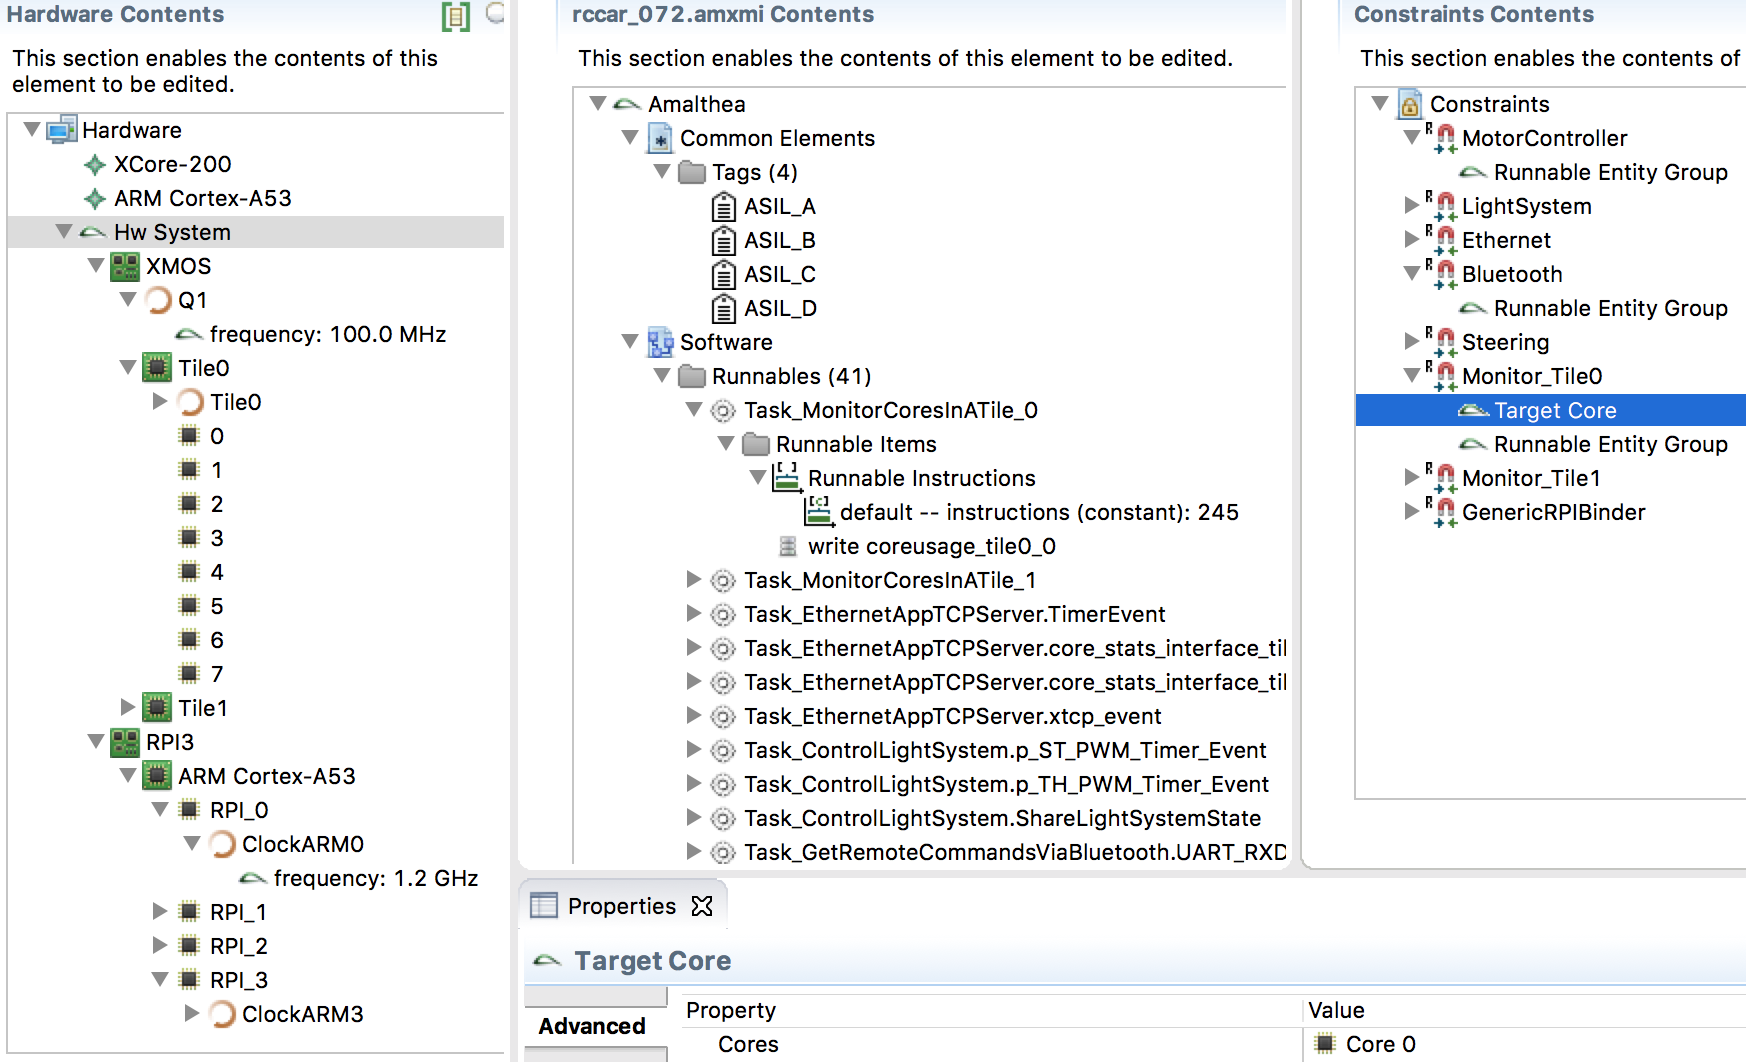
\includegraphics[scale=0.265]{images/models2.png}
	\caption{\label{fig:model}AMALTHEA hardware, software, and constraint models (excerpts) for the A4MCAR}
\end{figure}
\begin{figure*}[ht!]\centering
	\newcounter{groupcount}
	\pgfplotsset{
		legend style={at={(axis cs:21,0)},anchor=south west},
		draw group line/.style n args={5}{
			after end axis/.append code={
				\setcounter{groupcount}{0}
				\pgfplotstableforeachcolumnelement{#1}\of\datatable\as\cell{%
					\def\temp{#2}
					\ifx\temp\cell
					\ifnum\thegroupcount=0
					\stepcounter{groupcount}
					\pgfplotstablegetelem{\pgfplotstablerow}{X}\of\datatable
					\coordinate [yshift=#4] (startgroup) at (axis cs:\pgfplotsretval,0);
					\else
					\pgfplotstablegetelem{\pgfplotstablerow}{X}\of\datatable
					\coordinate [yshift=#4] (endgroup) at (axis cs:\pgfplotsretval,0);
					\fi
					\else
					\ifnum\thegroupcount=1
					\setcounter{groupcount}{0}
					\draw [
					shorten >=-#5,
					shorten <=-#5
					] (startgroup) -- node [anchor=base, yshift=0.5ex] {#3} (endgroup);
					\fi
					\fi
				}
				\ifnum\thegroupcount=1
				\setcounter{groupcount}{0}
				\draw [
				shorten >=-#5,
				shorten <=-#5
				] (startgroup) -- node [anchor=base, yshift=0.5ex] {#3} (endgroup);
				\fi
			}
		}
	}
	\begin{tikzpicture}%NO COMMENTS ALLOWED IN PGFPLOT VALUES
	\pgfplotstableread{
		X Gp D1 Name RPI C0 C1 C2 C3 C4 C5 C6 C7
		1 Sequential RPI Core0 100 0 0 0 0 0 0 0 0 
		2   Sequential RPI Core1 0 0 0 0 0 0 0 0 0
		3   Sequential RPI Core2 0 0 0 0 0 0 0 0 0
		4   Sequential RPI Core3 0 0 0 0 0 0 0 0 0
		5   Sequential XMOS Tile0 0 12.5 0 0 0 0 0 0 0 
		6   Sequential XMOS Tile1 0 0 0 0 0 0 0 0 0 
		8 Automatic RPI Core0 96 0 0 0 0 0 0 0 0
		9  Automatic RPI Core1 79.6 0 0 0 0 0 0 0 0
		10  Automatic RPI Core2 22.9 0 0 0 0 0 0 0 0
		11  Automatic RPI Core3 15.1 0 0 0 0 0 0 0 0
		12  Automatic XMOS Tile0 0 12.5 12.5 12.5 12.5 12.5 10 12.5 12.5 
		13  Automatic XMOS Tile1 0 12.5 12.5 12.5 12.5 0 0 0 0
		15  APP4MC RPI Core0 47 0 0 0 0 0 0 0 0
		16  APP4MC RPI Core1 34 0 0 0 0 0 0 0 0
		17  APP4MC RPI Core2 44 0 0 0 0 0 0 0 0
		18  APP4MC RPI Core3 60 0 0 0 0 0 0 0 0
		19  APP4MC XMOS Tile0 0 12.5 12.5 5 5 8 6 14 7 
		20  APP4MC XMOS Tile1 0 8 9 10 11 9 8 12 10 
	}\datatable
	\begin{axis}[
	axis lines*=left, ymajorgrids,
	width=16cm, height=6cm,
	ymin=0,
	ybar stacked,
	bar width=9pt,
	xtick=data,
	xticklabels from table={\datatable}{Name},
	xticklabel style={rotate=90,xshift=-7ex,anchor=mid east},
	draw group line={D1}{RPI}{RPI\,}{-7ex}{5pt},
	draw group line={D1}{XMOS}{XMOS\,}{-7ex}{5pt},
	draw group line={Gp}{Sequential}{Sequential}{-4ex}{7pt},
	draw group line={Gp}{Automatic}{Automatic}{-4ex}{7pt},
	draw group line={Gp}{APP4MC}{APP4MC}{-4ex}{7pt},
	after end axis/.append code={
		\path [anchor=base east, yshift=0.ex]
		(rel axis cs:0,0) node [yshift=-7ex] {Board}
		(rel axis cs:0,0) node [yshift=-4ex] {Distribution};
	}
	]
	
	\addplot table [x=X, y=RPI] {\datatable}; \addlegendentry{RPI}
	\addplot table [x=X, y=C0] {\datatable}; \addlegendentry{C0}
	\addplot [teal!80!black,fill=teal!50!white] table [x=X, y=C1]{\datatable}; \addlegendentry{C1}
	\addplot [violet!80!black,fill=violet!50!white] table [x=X, y=C2]{\datatable}; \addlegendentry{C2}
	\addplot [pink!80!black,fill=pink!50!white] table [x=X, y=C3]{\datatable}; \addlegendentry{C3}
	\addplot [brown!80!black,fill=brown!50!white] table [x=X, y=C4]{\datatable}; \addlegendentry{C4}
	\addplot [cyan!80!black,fill=cyan!50!white] table [x=X, y=C5]{\datatable}; \addlegendentry{C5}
	\addplot [lightgray!80!black,fill=lightgray!50!white] table [x=X, y=C6]{\datatable}; \addlegendentry{C6}
	\addplot [orange!80!black,fill=orange!50!white] table [x=X, y=C7]{\datatable}; \addlegendentry{C7}
	\end{axis}
	\end{tikzpicture}
	\vspace{-20pt}
	\caption{Core utilization in \% (y-axis) for sequentail, automatic, and APP4MC distribution}
	\label{fig:dischart}
\end{figure*}
Apart from the constraints, software and hardware descriptions are required. While the hardware model is created manually, a C/CPP parser was used to receive necessary AMALTHEA software model data, i.e. runnables, labels, label accesses, activations, runnable calls, \underline{I}nterrupts \underline{S}ervice \underline{R}outines (ISRs), Semaphores, and more for the Raspberry Pi (RPI) implementations. Excerpts of those models are shown in Figure~\ref{fig:model} in form of an APP4MC screenshot. From left to right, the hardware, software and constraint models are shown, whereas the lower part illustrates the properties view of the selected \textit{Target Core} property providing the reference to \textit{Core 0} of the hardware model. This means, that the runnables referenced in the \textit{Runnable Entity Group} of this constraints will be mapped to the \textit{Core 0} within the parallelization processes. 

Runnables of the RPI can be derived from a \textit{LLVM} \cite{llvm} parser (created 247 runnables for a basic application with driving controls only) but our use case model features RPI runnables derived from a python script since the hierarchical structure of \textit{LLVM} runnables has not been investigated yet. XMOS implementations were modeled on upon threads only, that correspond tasks. Those count 30 in total and instruction deviations are received via counting assembler instructions and using individual profiling scripts.  

%TODO insert how instructions of XMOS threads were found out
%The created scripts or applications need to be modeled precisely with APP4MC in order to get more accurate results. 
More precisely, the Linux OS provides a set of important kernel-level tools as well as methods to analyze processes, threads, and binaries. Consequently, we use those to model the implementations and transform them to Amalthea models. Since the amount of runnables, i.e. smallest executable units derived from functions, %often reaches beyond 100,
exceeds 100 in most cases, the required transformation is done automatically by a parser. Therefore, we use the tool '\texttt{objdump}' due to its capability to derive disassembled runnables from binary files created from C or C++ files. While this approach is acutely straight forward, deriving instructions, deadlines, or WCET has to be addressed by specific profiling tools that handle binary object disassembly. For this purpose the '\texttt{perf}' tool fits our need most and has been integrated into a script to derive the required instructions. 
Furthermore, via accessing the kernel folder '\texttt{proc}', we check each processes' used memory, libraries, variables, and functions and set affinity constraints in APP4MC to keep some specific functions from being separated during partitioning or mapping processes. 

%The first required step that is needed in order to properly model the runnables and tasks is getting the proper number of instructions by either looking at disassembly of binary objects or using profiling tools. 
%In order to profile the dynamic processes, which are one of the greatest parts in our application, the tool 'perf' has been used. 
%A linux system bash script has been created in order to get the dynamical instructions by making use of this tool.
%One could also make use of the kernel folders in Linux such as 'proc' in order to define constraints for the processes while modeling them in APP4MC.
%Furthermore, the runnables within C/C++ applications are disassembled and analyzed by using the tool 'objdump', which creates disassembled runnables from binary files.
Linux provides other methods such as '\texttt{top}' and '\texttt{taskset}', which are also crucial to the development of multi-core systems. The tool '\texttt{top}' is used for the process monitoring, whereas the method '\texttt{taskset}' realizes thread to core mapping in order to manage the multi-core distribution provided by APP4MC.
%In the A4MCAR, the aforementioned tools are used in order to manage a multi-process system distributed on multiple cores.
The specific mapping on the A4MCAR is finally considered automatically by a generated C file from APP4MC that distributes the tasks using Linux's '\texttt{taskset}'.

Before the partitioning and mapping processes can be configured and executed, one of the most challenging key property has to be added to runnables, i.e. the above mentioned affinity, allocation, and safety constraints.
%TODO  constraints modeling

%EQUATION-----------------------------------------------
%\begin{equation}
%\label{Eq_1}
%\lambda_i = \lim \frac{1}{p} \sum_{t=1}^p \ln \frac{|w_i (t)|}{|w_i (t-1)|}
%\end{equation}

%TODO maybe skip the following chapter
%\section{Precise modeling and Software Parallelization}
%\label{sec:impl}

%FIGURE-----------------------------------------------
%\begin{figure}[bth]
%\centering
%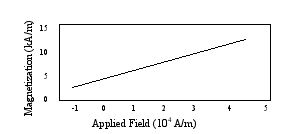
\includegraphics[scale=0.6]{images/Fig1.png}
%\caption{\label{Fig_Magnet}Magnetization as a function of applied field. Note 
%how the caption is centered in the column.}
%\end{figure}

%TABLE-----------------------------------------------
%\begin{table}[htb]
%\caption{Table Type Styles}
%\label{Table_I}1
%\centering
%\begin{tabular}{|p{1.2cm}|p{1.5cm}|p{1.5cm}|p{1.5cm}|}
%\hline
%\multirow{2}{1.2cm}{\textbf{Type Size (pts.)}} & \multicolumn{3}{|c|}{\textbf{Appearance}}\\
%\cline{2-4}
% & \textbf{\textit{Regular}}&\textbf{\textit{Bold}}&\textbf{\textit{Italic}}\\
%\hline
%8 & References, table header, footnotes, text subscripts, and superscripts &&\\
%\hline
%\end{tabular}
%\end{table}

\section{Evaluation}
\label{sec:eval}
Figure \ref{fig:dischart} shows results of three different software distribution scenarios on the A4MCAR obtained from separate utilization tracker threads. \\
For clarity purposes, the XMOS logical cores were combined to the corresponding tiles since their separation would result in less clarity as well as lessen the physical accordance. Hence, each colored rectangle on a XMOS tile can consume up to 12,5\% maximal tile utilization, such that a tile is only fully utilized if all 8 cores fully express 12,5\% core utilization.

The distributed sequential parallelization (left part of Figure \ref{fig:dischart}) shows that each board (RPI \& XMOS) has one fully utilized processing unit. Consequently, applications and tasks can hardly meet their deadlines and execute with very low throughput. In contrast to that, when using the Linux \underline{C}ompletely \underline{F}air \underline{Q}ueuing (CFQ) scheduler without explicitly defining priority or scheduling classes %more info required?
on the RPI as well as the round robin scheduler on the XMOS via \texttt{par} statements, one can experience great benefits due to concurrent progressing on both hardware units (see mid part of Figure \ref{fig:dischart}). Nevertheless, for this case programmers still need to manually separate the real time applications from the non-critical programs and map them to the corresponding processing elements (critical programs to the XMOS, non-critical to the RPI). It is important to note here, that the non-critical tasks still have deadlines to meet in order to assess effectiveness, i.e. that results are produced within a limited time period predefined by requirements.
%TODO maybe explain the following comments
%If your code is in the processor cache it will execute in one clock, or whatever it takes.
%If you code needs to fetched from cache it might take 10 times longer, say.
%I don't know how many levels of cache there are, but for every level we can say 10 times longer again,
%If your code is not in any cache it will have to be fetched from RAM. Another ten ties longer.
%Your code may not even be in RAM, it may have been swapped out a swap file on disk, That's 100s or thousands of times longer.
%Finally, if the Linux kernel decides to do something else your code will be suspended for what could be a long time, perhaps forever.
%So, unless you are writing code "to the bare metal" with no operating system underneath it and you know how you code fits into the caches and how it thrashes the caches at run time you have no chance of determining the execution time of any particular instruction.

However, as pointed out earlier in this paper, the automatic distributions are not always the prior choice when targeting efficiency. Deadlines may be met comprehensively (the effect is the same), but long slack times waste processing cycles that could be spent otherwise. The APP4MC distribution (right part of Figure \ref{fig:dischart}) not only considers any types of constraints but also can be configured to balance load as much as possible such that for instance the total frequency (here on the RPI) could be scaled down to safe energy. Assuming a global \underline{D}ynamic \underline{V}oltage and \underline{F}requency \underline{S}caling (DVFS) feature on the RPI, we measured up to 9\% less energy consumption when commonly reducing the CPU frequencies from 1200MHz to 800MHz while still meeting all deadlines.  %TODO real measurements required; also assumption: DFVS global, since Linus does not allow CPUinfo_min_freq per-core
In addition, all real time tasks running on the XMOS could be relieved from some load, such that tile utilization could be reduced and task response times occur even earlier than at the automatic distribution. 
It has to be added here, that there are various configuration possibilities for both the partitioning and the mapping. Each configuration may result in different outcomes. Figure \ref{fig:dischart} shows results obtained from critical path partitioning whereas the global critical path is used to define the schedule length for all other tasks and activation consideration switched on. The mapping process has been configured to use an Integer Linear Programming (ILP) solver for load balancing with the default values for max gap, iterations, etc. 
%in parallel and distributed systems like
\section{Related Work}
\label{sec:relatedWork}
With the advent of multi-core or many-core hardware in embedded systems, a lot of work dealing with the efficient distribution of software to the respective cores with regard to specific constraints has been published. Socci et al. \cite{Socci2015} provide an algorithm for multi-processor scheduling of mixed criticality task graphs in synchronous systems through precedence constraints. 
Xiao et al. \cite{Xiao2016} focus on minimizing the energy consumption by scheduling parallel application towards heterogeneous distributed environments based on energy consumption constraints, while Liang et al. \cite{LiXi13} propose an algorithm for reducing the energy consumption of high performance clusters via precedence
constrained without increasing the schedule length. In contrast to the prementioned work, our approach takes several kinds of design constraints, e.g. affinity, allocation or ASIL constraints, into account.

In \cite{Kritikakou2014}, Kritikakou et al. describe a WCET analyzer that has similarities to how we receive instruction parameters. However, their main focus is an extensive modeling technique required for design-time analysis that considers both critical and non-critical tasks to target better resource utilization. This graph based design is equivalent to graphs in APP4MC whereas some additional notation are used to derive conditions, hierarchies, loops, calls and more. While those additions can be added to improve WCET reasoning, the focus of heterogeneous systems is the advancement of this paper.

In \cite{cheramy2014}, several scheduling approaches are provided and described along python implementations. Those can be subject to further integration to APP4MC for the purpose of advanced timing and resource management analyses. Their precise utilization with the A4MCAR can be investigated in order to check for more effective software distribution results.
\section{Conclusion}
\label{sec:concl}
Within this paper, we successfully validated that using APP4MC for efficient mixed-critical software parallelization to distributed heterogeneous systems eases development processes on various levels. Error prone and time consuming manual software distribution can be avoided and utilizing APP4MC results even outperforms sequential and automatic approaches provided by the operating system regarding load balancing and energy consumption. While the constraint modeling still requires certain efforts, it considers crucial requirements emerging from timing, safety, or security demands that are inevitable in modern industrial developments. Our experiments among the A4MCAR example show that load balancing, energy consumption (9\%), and system responsiveness (less deadline proximity) can be significantly improved when using APP4MC features.

Upcoming work addresses advanced WCET reasoning, utilizing preemtiveRT\cite{preemptrt} on the Linux kernel, and advanced software component (SWC) based partitioning in order to extend parallelism utilization by less runnable pairing constraints and the possibility of merging SWCs to create even less slack or idle times during system execution. Furthermore, implementing different scheduling algorithms and accessing the Linux kernel to adjust scheduling properties is of major interest to gain more precise real time control on the RPI. Finally, applying resource management research presented in \cite{HIS2017date} to the A4MCAR in order to further reduce tasks response times via specific runnable schedule tables could improve current memory management respectively resource utilization.
%TODO maybe more Amalthea paper?
\section*{Acknowledgment}
The authors would like to express their appreciation to the AMALTHEA4public consortium for sharing experience, knowledge, and expertise. %Special thanks to 
\enlargethispage{20pt}
\bibliographystyle{IEEEtran}
\bibliography{ref}
\end{document}